\documentclass[sn-mathphys-num]{sn-jnl}
\usepackage{graphicx}%
\usepackage{multirow}%
\usepackage{amsmath,amssymb,amsfonts}%
\usepackage{amsthm}%
\usepackage[mathscr]{mathalpha}%
\usepackage[title]{appendix}%
\usepackage{xcolor}%
\usepackage{textcomp}%
\usepackage{manyfoot}%
\usepackage{booktabs}%
\usepackage{algorithm}%
\usepackage{algorithmicx}%
\usepackage{algpseudocode}%
\usepackage{listings}%
\usepackage{lmodern}
\usepackage{tabularx}


\raggedbottom
\begin{document}
\title[Article Title]{Application of LSTM Neural Networks and Complex Network Analysis for Earthquake Forecasting in Colombia}

%%=============================================================%%
%% GivenName	-> \fnm{Joergen W.}
%% Particle	-> \spfx{van der} -> surname prefix
%% FamilyName	-> \sur{Ploeg}
%% Suffix	-> \sfx{IV}
%% \author*[1,2]{\fnm{Joergen W.} \spfx{van der} \sur{Ploeg} 
%%  \sfx{IV}}\email{iauthor@gmail.com}
%%=============================================================%%

\author*[1]{\fnm{Santiago} \sur{Giraldo}}\email{giraldo.santiago@correounivalle.edu.co.com}

\author[2]{\fnm{Daniel} \sur{León}}\email{daniel.leon@correounivalle.edu.co}
\equalcont{These authors contributed equally to this work.}

\author[3]{\fnm{Victor} \sur{Bucheli}}\email{victor.bucheli@correounivalle.edu.co}
\equalcont{These authors contributed equally to this work.}

\affil*[1,2,3]{\orgdiv{Escuela de Ingeniería de Sistemas}, \orgname{Universidad del Valle}, \orgaddress{\street{13th st.}, \city{Cali}, \postcode{760033}, \state{Valle del Cauca}, \country{Colombia}}}


\abstract{
    Earthquakes are unpredictable and high-risk events that can cause significant human casualties and infrastructure damage. In recent years, there has been a surge in research on earthquake forecasting using machine learning and neural networks, yielding impressive results. This study addresses the earthquake forecasting problem by applying Long Short-Term Memory (LSTM) Neural Networks to historical seismic events along Colombia's Pacific coast, using data from the United States Geological Survey. We analyzed the seismic catalog over time, incorporated complex network features for each dataset, and trained multiple LSTM neural networks with hyper-parameter tuning. Features such as latitude, longitude, magnitude, days elapsed between events, and complex network properties were used. Models utilizing only earthquake features achieved 60-70\% accuracy for 2-quantile classification, while models incorporating complex network features achieved similar accuracy for 3-quantile classification. These results are promising and offer a new perspective on the use of complex networks in earthquake forecasting.
}

\keywords{Earthquake Forecasting, LSTM Neural Networks, Machine Learning, Complex Networks}
\maketitle
\section{Introduction}\label{introduction}

Earthquakes are classified a high risk event due to their unexpected nature and the limited time available to take preventive actions. Furthermore, the earthquakes may cause the human casualties and infrastructure damage. Over the past few years, numerous papers have explored the use of machine learning algorithms and neural networks for earthquake forecasting \cite{banna_application_2020, florido_earthquake_2016, mignan_neural_2020, jiao_artificial_2020, galkina_machine_nodate, kong_machine_2019}. The growing interest in the use of machine learning has been documented, as well as the use of artificial intelligence to forecast seismic events, indicating future work and various challenges to be addressed.

One approach involves the application of deep neural networks to learn from data directly to identify complex patterns. However, forecasting features such as magnitude is limited by the lack of events that exceed certain thresholds. A more promising approach uses a set of different characteristics and regions as input to the neural network in a moving window of time \cite{wang_earthquake_2020}.

Some of the documented features in literature are magnitude, frequency of events \cite{han_medium-_1997,de_falco_seismicity_2000,bodri_neural-network_2001,wang_support_2006,sri_lakshmi_model_2009}, occurrence of aftershocks \cite{lin_forecast_2002}, probability of detection and rate of false alarms \cite{panakkat_neural_2007} , geomagnetic field variation, soil temperature and relative humidity \cite{suratgar_magnitude_2008}, seismic indicators \cite{panakkat_recurrent_2009}, location \cite{veri_earthquake_2012}, Gutenberg-Richter b-value \cite{morales-esteban_earthquake_2013,reyes_neural_2013,asenciocortes_earthquake_2018}, gravity, georesistivity and water level \cite{cai_anomaly_2019}, elapsed days, mean magnitude, mean time between characteristic events, coefficient of variation of the mean time \cite{banna_attention-based_2021}, and electronic signals captured on seismographs \cite{bose_preseis_2008,lakkos_neural_1994,rovithakis_neural_2000,ifantis_support_2003,radeva_real-time_2005,bernardo-torres_one-step_2009}.

Artificial intelligence and machine learning algorithms are powerful tools for addressing a wide range of classification and forecasting problems. They have the potential to learn from hidden patterns within the provided data \cite{kong_machine_2019}. As seen in \cite{kong_machine_2019, bose_preseis_2008}, their application in earthquake forecasting is useful for risk assessment and early prevention. 

In \cite{jiao_artificial_2020}, it is stated that studies in seismology are carried out for the following objectives: actions to reduce long-term disasters generated by earthquakes, preparation and adjustment to disasters, disaster response strategies, and post-disaster recovery planning. According to Satriano et al. \cite{satriano_earthquake_2011}, information systems focused on the early warning of seismological events must quickly and reliably provide information on different parameters such as location, time, and size to improve emergency response. Espinosa et al. \cite{espinosa-aranda_evolution_2009} mention that the Mexican SAS (seismic alert system), an early warning system implemented in Mexico, has allowed seismic waves to be detected up to 60 seconds in advance, a time frame that allows security procedures to be executed to protect equipment susceptible to damage, such as power plants, computer systems, and communication networks.

Additionally, there has been increasing interest in representing data through graphs, as complex relationships can be modeled using nodes and edges \cite{chami_machine_2021}. Earthquakes can be modeled as a complex network, representing locations as nodes and sequences as edges \cite{leon_modeling_2018}. Learning from these structures has been successfully applied in particle interaction, recommendation systems, molecular properties, natural language processing, and other fields \cite{grattarola_graph_2020}.

In his work, León et al. \cite{leon_modeling_2018} showed that representing seismological events as complex network helps understand of seismicity in a region and unravel the relationships among these events. Earthquake networks are based on the temporal sequence of events and their specific locations. Different network features, such as path length, degree distribution, and clustering, help define the relationships between events, hubs, and small-world network properties. For example, \textbf{Path length} measures the average shortest path between nodes in the network, indicating how quickly information (or seismic activity) can spread through the network \cite{newman_2010}. \textbf{Degree distribution} describes the probability distribution of the degrees over the entire network, helping to identify nodes with a high number of connections, which may act as critical points in the network \cite{barabsi_2009}. \textbf{Clustering coefficient} measures the degree to which nodes in a graph tend to cluster together, providing insights into the local interconnectedness of the network \cite{watts_1998}. 

In this work, we wanted to answer whether incorporating network features can enhance the performance of LSTM models for earthquake forecasting. LSTM models have been widely used to model temporal data and earthquake forecasting \cite{lai_modeling_2018, cai_anomaly_2019,banna_attention-based_2021,wang_earthquake_2020, nazaria_predicting_2021}. By processing earthquake data from Colombia and training LSTM neural network models, we found that models achieved 60-70\% accuracy for 2-quantile classification and similar accuracy for 3-quantile classification when network features were included. These results indicate that complex network features can indeed improve earthquake forecasting accuracy.

\section{Methods}\label{methods}

In this section, we take a look at the training and test data, and the steps to generate the earthquake features used later for training.

The earthquake events used in this study were obtained from the U.S. Geological Survey (USGS) for the Colombian region, with latitudes ranging from -0.132° to 9.796° and longitudes from -80.343° to -72.466°. The events are plotted by magnitude and depth in \textbf{Figure \ref{fig1}}. The retrieved dataset contained 5462 events since 1975, which was reduced to 4042 events after processing. The data cleaning process involved removing empty values, converting string values to numerical values for certain features, and filtering out events that were not validated by multiple sources, had missing data points, or had zero values. The selected events were of the mb type, representing the body wave magnitude, and included the depth of the event.

\begin{figure}[H]
    \includegraphics[width=0.49\textwidth]{img/mag.png}
    \includegraphics[width=0.49\textwidth]{img/depth.png}
    \caption{Earthquake events visualization by Magnitude (left) and Depth (right)}\label{fig1}
\end{figure}
\unskip

\subsection{Earthquake Networks}\label{earthquake_networks}
Following the methodology proposed by Leon et al. \cite{leon_modeling_2018}, constructing an Earthquake Complex Network involves dividing the selected geographical area into a grid of cells, we'll call them nodes from now on, each representing a specific distance in kilometers. Sequential earthquake events are then used to establish connections between these nodes, forming the network. In \ref{fig2} we can see a diagram of the process of creating an earthquake network.

\begin{figure}[H]
    \begin{center}
        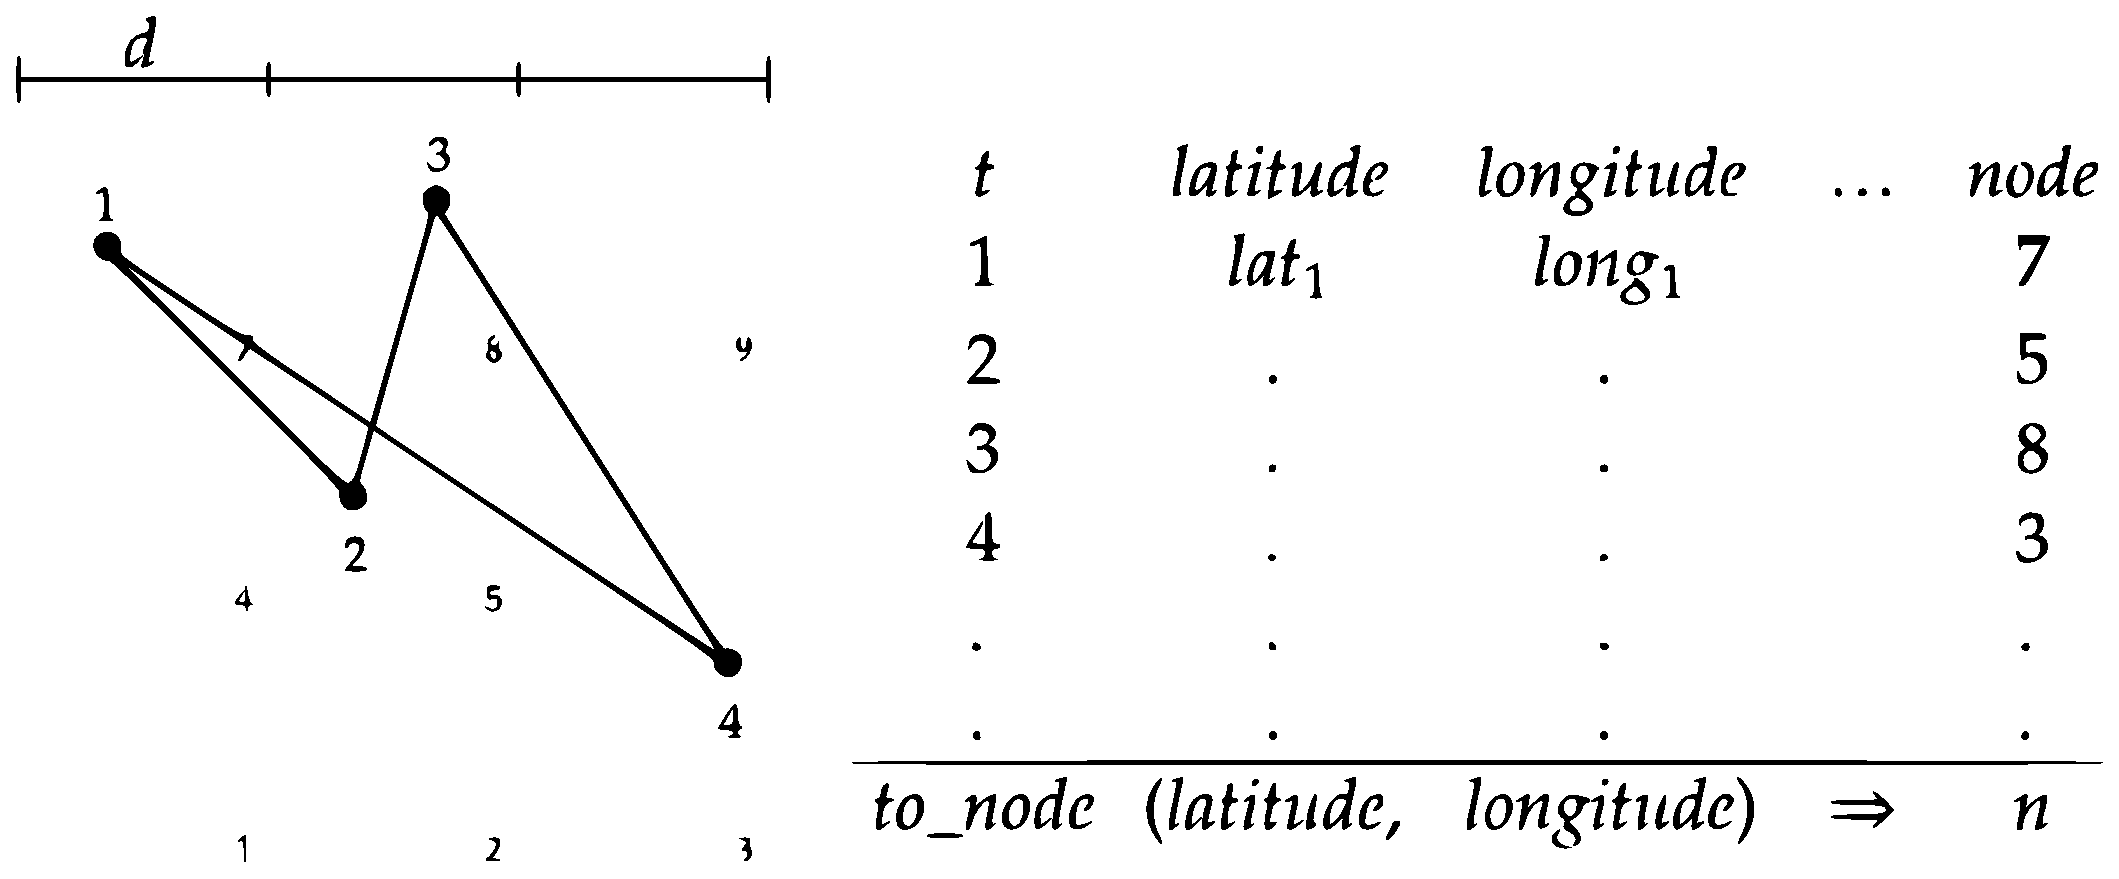
\includegraphics[width=0.7\textwidth]{img/eqnetwork.eps}
        \caption{Quick overview of the creation of an earthquake network. A geographical region is divided into nodes of equal size in kilometers, then each event is clasified in each node by its latitude and longitude, we later connect each node by the time sequence of the events. We can observe nodes 7, 5, 8, 3 are connected in that order, first (7,5), then (5,8), and finally (8,3).
        } \label{fig2}
    \end{center}
\end{figure}
\unskip

\subsection{Dataset}\label{dataset}
After processing and cleaning the data, we assigned each earthquake event to a node based on its geographical location. We then normalized the features to ensure they were consistent and comparable across the dataset. To analyze the data at different levels of detail, we divided the features into 2, 3, and 4 quantiles. Next, we created the sequences needed for training the LSTM network. This involved generating rolling windows of events, where each window contained a sequence of features used as input to the model, and a feature of the following event as the target.

\begin{table}[ht]
    \caption{Dataset Statistics}\label{tab1}
    \begin{tabular}{@{}llllllll@{}}
        \toprule
        Feature   & Min    & Max    & Median & Mean   & SD    & Variance & Range  \\
        \midrule
        Latitude  & -0.13  & 9.79   & 6.73   & 5.73   & 2.08  & 4.31     & 9.92   \\
        Longitude & -80.34 & -72.47 & -75.68 & -75.55 & 2.49  & 6.20     & 7.88   \\
        Depth     & 0.00   & 436.50 & 68.10  & 89.68  & 65.50 & 4290.78  & 436.50 \\
        Magnitude & 0.00   & 7.80   & 4.40   & 4.19   & 0.99  & 0.97     & 7.80   \\
        \botrule
    \end{tabular}
    \footnotetext{
        Resume of the features used in the dataset, we can see the minimum, maximum, median, mean, standard deviation, variance, and range of the features.
    }
\end{table}
\unskip

Following the methodology proposed by Lin et al. \cite{lai_modeling_2018}, multivariate time-series forecasting involves using a rolling window approach. In this context, the input to the model is a sequence of values \( \{y_1, y_2, \ldots, y_l\} \), and the output is the value \( y_{l+l} \), where \( l \) represents the lookback number of events. We applied this approach to the earthquake data, using the features within each window as inputs to the LSTM network, then selecting features of the following event as the target.

The sequences were explored according to the lookback parameter, we generated different matrices of size \( (S, L) \) resulting in a dataset of size \( (N, S, L)\). The following figure shows the structure of the dataset for the LSTM network.

\begin{figure}[H]
    \begin{center}
        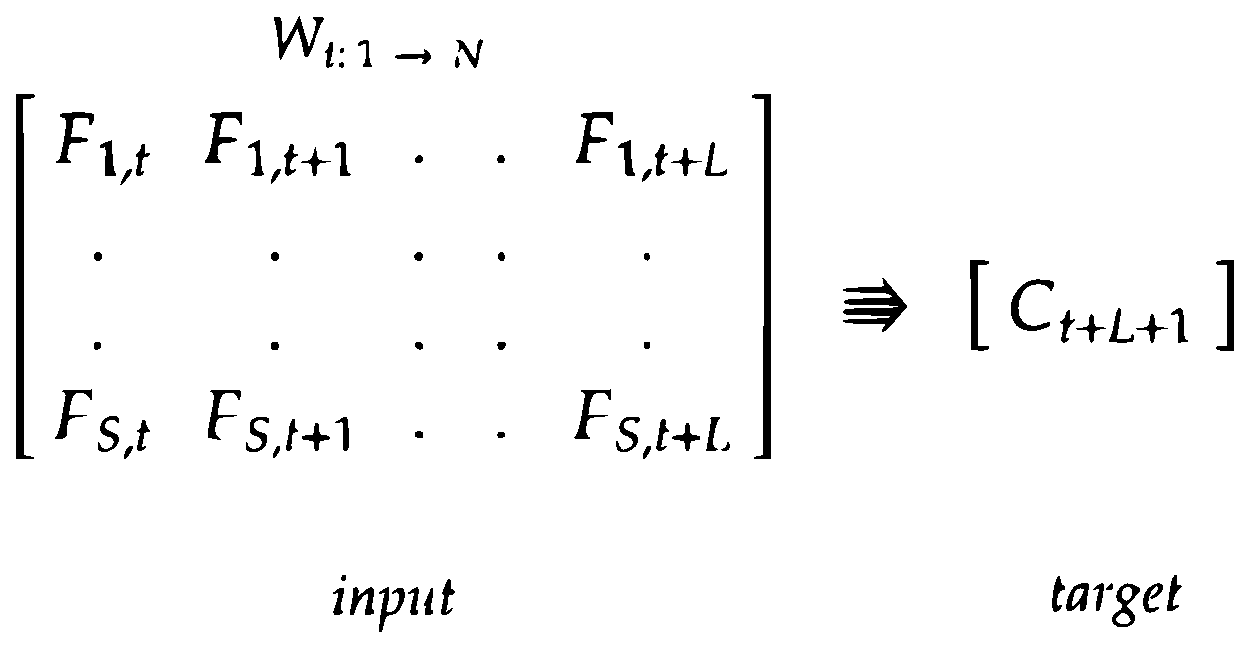
\includegraphics[width=0.6\textwidth]{img/dataset.eps}
        \caption{Dataset for the LSTM neural network.\label{fig3}}
    \end{center}
\end{figure}

In the figure above, we can identify the variables F, S, L, W, t, N, and C where:

\begin{enumerate}
    \item \( F_{S,L} \) is a time-series sequence of a feature
    \item S is the sequence identifier that matches the number of features in the catalog plus the augmented features
    \item L is the lookback or length of the sequence
    \item W is the window of events with time index t, which ranges from 0 to N, where N is the total number of events minus the lookback
    \item C is the class of the target feature that follows the previous sequence
\end{enumerate}


To calculate the complex network properties, as discussed in Section \ref{earthquake_networks}, we constructed a network for each moving window of earthquake events. The geographical area was divided into a grid of nodes, with each node representing a specific distance in kilometers. We experimented with different node distances of 30, 50, and 100 kilometers.

For each moving window, we built the corresponding network by connecting nodes based on the sequential occurrence of earthquake events. The edges between nodes were established according to the temporal order of events, forming a directed graph. Once the network was constructed, we calculated several complex network properties to capture the structural characteristics of the network. These properties included:

\begin{itemize}
    \item \textbf{Degree Centrality}: Measures the number of direct connections a node has. It helps identify the most connected nodes within the network.
    \item \textbf{Clustering Coefficient}: Indicates the degree to which nodes tend to cluster together. It provides insight into the local interconnectedness of the network.
    \item \textbf{Betweenness Centrality}: Quantifies the number of times a node acts as a bridge along the shortest path between two other nodes. It highlights nodes that play a critical role in connecting different parts of the network.
    \item \textbf{Closeness Centrality}: Reflects how close a node is to all other nodes in the network. It measures the average shortest path length from a node to all other nodes.
    \item \textbf{PageRank}: An algorithm originally used by Google to rank web pages. It assigns a probability distribution representing the likelihood of visiting each node, considering the structure of the network.
\end{itemize}

These network features were then incorporated into the LSTM neural network models as additional input features. By combining traditional earthquake features with complex network properties, we aimed to enhance the model's ability to capture the underlying patterns and relationships within the seismic data. The results of these experiments are presented in Section \ref{results}, demonstrating the impact of incorporating complex network analysis on earthquake forecasting accuracy.

\section{Results}\label{results}

In this section, we present the results of the LSTM neural networks trained with the earthquake data. We trained multiple models tuning for hyperparameters, including the number of LSTM layers, hidden size, learning rate, and maximum number of epochs. We also included the complex network features in the training process to evaluate their impact on the forecast results.

Multiple experiments were conducted as shown in Table \ref{tab2}. We categorized the target magnitude into 2, 3, and 4 quantiles as follows:
\begin{enumerate}
    \item 2 quantiles: The feature is divided into two sections, each containing 50\% of the data, corresponding to the categories low and high.
    \item 3 quantiles: The feature is divided into three sections, containing data from 0\%-33.3\%, 33.3\%-66.6\%, and 66.6\% onwards, corresponding to the categories low, medium, and high.
    \item 4 quantiles: The feature is divided into four sections, each containing 25\% of the data, corresponding to the categories low, low-medium, medium-high, and high.
\end{enumerate}

It was observed that the best model with 2 quantiles achieved 64\% accuracy, followed by the best model with 3 quantiles with 46\% accuracy, and the model with 4 quantiles with 41\% accuracy.

\begin{sidewaystable}
    \caption{Results of the LSTM Neural Networks}\label{tab2}
    \begin{tabular}{@{}lllllllllll@{}}
        \toprule%
        loss     & test loss & lookback & test size & batch size & hidden size & lstm layers & lr    & max epochs & accuracy & quantiles \\
        \midrule
        1014.889 & 449.927   & 33       & 0.176     & 2          & 80          & 4           & 0.000 & 60         & 0.640    & 2         \\
        823.150  & 733.873   & 144      & 0.282     & 2          & 97          & 2           & 0.000 & 25         & 0.634    & 2         \\
        133.589  & 690.542   & 102      & 0.268     & 14         & 129         & 8           & 0.001 & 19         & 0.606    & 2         \\
        126.626  & 367.758   & 147      & 0.139     & 18         & 144         & 7           & 0.000 & 58         & 0.582    & 2         \\
        \midrule
        409.568  & 525.436   & 78       & 0.117     & 7          & 77          & 4           & 0.002 & 45         & 0.463    & 3         \\
        150.548  & 1386.181  & 54       & 0.270     & 12         & 105         & 2           & 0.003 & 48         & 0.447    & 3         \\
        38.531   & 1464.909  & 124      & 0.119     & 19         & 33          & 4           & 0.001 & 33         & 0.430    & 3         \\
        165.997  & 1109.243  & 13       & 0.263     & 19         & 113         & 2           & 0.000 & 53         & 0.413    & 3         \\
        \midrule
        405.722  & 1245.538  & 65       & 0.227     & 8          & 129         & 5           & 0.000 & 25         & 0.411    & 4         \\
        173.115  & 848.971   & 106      & 0.134     & 19         & 101         & 2           & 0.001 & 28         & 0.397    & 4         \\
        266.301  & 790.450   & 148      & 0.158     & 16         & 76          & 5           & 0.000 & 52         & 0.387    & 4         \\
        249.980  & 902.233   & 136      & 0.156     & 15         & 22          & 2           & 0.008 & 36         & 0.382    & 4         \\
        \botrule
    \end{tabular}
    \footnotetext{
        Top 4 models for 2 quantiles, 3 quantiles, and 4 quantiles, respectively. The table shows the loss, test loss, lookback, test size, batch size, hidden size, LSTM layers, learning rate, maximum epochs, accuracy, quantiles, network features, and node size.
    }
\end{sidewaystable}
\unskip

To incorporate complex network features into the training process, we calculated network properties for each window of events. The LSTM network was then trained using both earthquake features and network properties, with quantiles and node sizes varied for each case, and the selection of network properties determined through hyperparameter tuning. The results are presented in Table \ref{tab3}. The best model with 2 quantiles achieved 65\% accuracy, followed by the best model with 3 quantiles at 48\% accuracy, and the best model with 4 quantiles at 43\% accuracy.

\begin{sidewaystable}
    \caption{Results of the LSTM Neural Networks with Network Features}\label{tab3}
    
    \begin{tabularx}{\textwidth}{@{}XXXXXXXXXXXll@{}}
        \toprule
        loss     & test loss & lookback & test size & batch size & hidden size & lstm layers & lr    & max epochs & accuracy & quantiles & network features & node size \\
        \midrule
        112.576  & 433.087   & 82       & 0.173     & 18         & 20          & 6           & 0.003 & 39         & 0.648    & 2         & betweenness      & 30        \\
        114.802  & 248.123   & 104      & 0.103     & 19         & 133         & 7           & 0.004 & 18         & 0.647    & 2         & clustering       & 30        \\
        513.069  & 273.118   & 122      & 0.110     & 4          & 106         & 2           & 0.001 & 58         & 0.644    & 2         & degree           & 30        \\
        \midrule
        705.396  & 1115.538  & 149      & 0.276     & 4          & 19          & 4           & 0.002 & 38         & 0.473    & 3         & degree           & 30        \\
        312.249  & 985.935   & 145      & 0.239     & 9          & 64          & 2           & 0.008 & 18         & 0.465    & 3         & betweenness      & 30        \\
        404.635  & 416.466   & 79       & 0.102     & 9          & 138         & 9           & 0.000 & 55         & 0.464    & 3         & betweenness      & 30        \\
        \midrule
        269.973  & 1138.736  & 105      & 0.225     & 14         & 73          & 8           & 0.001 & 38         & 0.408    & 4         & clustering       & 30        \\
        527.298  & 1006.915  & 75       & 0.166     & 6          & 68          & 2           & 0.003 & 30         & 0.391    & 4         & clustering       & 30        \\
        212.685  & 813.492   & 148      & 0.161     & 19         & 64          & 6           & 0.000 & 67         & 0.375    & 4         & pagerank         & 30        \\
        \midrule
        1063.339 & 456.658   & 13       & 0.152     & 2          & 36          & 3           & 0.007 & 12         & 0.651    & 2         & pagerank         & 50        \\
        128.613  & 602.748   & 147      & 0.249     & 14         & 69          & 4           & 0.000 & 54         & 0.647    & 2         & pagerank         & 50        \\
        249.543  & 417.286   & 82       & 0.162     & 8          & 12          & 2           & 0.001 & 45         & 0.640    & 2         & pagerank         & 50        \\
        \midrule
        402.819  & 1202.975  & 36       & 0.300     & 7          & 124         & 4           & 0.002 & 52         & 0.487    & 3         & closeness        & 50        \\
        406.882  & 1182.266  & 139      & 0.293     & 7          & 101         & 7           & 0.000 & 66         & 0.480    & 3         & pagerank         & 50        \\
        192.634  & 1022.804  & 20       & 0.184     & 11         & 80          & 2           & 0.004 & 32         & 0.464    & 3         & betweenness      & 50        \\
        \midrule
        308.907  & 959.463   & 137      & 0.194     & 13         & 70          & 5           & 0.001 & 45         & 0.432    & 4         & closeness        & 50        \\
        350.506  & 836.819   & 10       & 0.165     & 12         & 116         & 3           & 0.000 & 39         & 0.429    & 4         & clustering       & 50        \\
        664.843  & 1094.966  & 10       & 0.212     & 6          & 117         & 2           & 0.000 & 46         & 0.409    & 4         & closeness        & 50        \\
        \midrule
        294.545  & 355.232   & 49       & 0.142     & 7          & 128         & 6           & 0.000 & 26         & 0.671    & 2         & betweenness      & 100       \\
        297.019  & 685.403   & 18       & 0.280     & 6          & 114         & 4           & 0.001 & 57         & 0.662    & 2         & closeness        & 100       \\
        720.330  & 352.685   & 84       & 0.145     & 3          & 56          & 6           & 0.003 & 39         & 0.657    & 2         & pagerank         & 100       \\
        \midrule
        254.312  & 846.157   & 94       & 0.202     & 11         & 62          & 4           & 0.001 & 11         & 0.467    & 3         & betweenness      & 100       \\
        191.379  & 1270.860  & 140      & 0.289     & 12         & 51          & 2           & 0.001 & 23         & 0.466    & 3         & clustering       & 100       \\
        183.231  & 497.836   & 116      & 0.106     & 16         & 27          & 5           & 0.000 & 23         & 0.461    & 3         & degree           & 100       \\
        \midrule
        696.927  & 832.365   & 53       & 0.163     & 6          & 140         & 8           & 0.000 & 41         & 0.417    & 4         & pagerank         & 100       \\
        300.884  & 1110.282  & 13       & 0.219     & 13         & 35          & 3           & 0.004 & 62         & 0.403    & 4         & degree           & 100       \\
        231.743  & 1483.400  & 128      & 0.296     & 16         & 140         & 6           & 0.004 & 32         & 0.381    & 4         & closeness        & 100       \\
        \botrule
    \end{tabularx}
    \footnotetext{
        Top 4 models for 2 quantiles, 3 quantiles, and 4 quantiles, respectively. The table shows the loss, test loss, lookback, test size, batch size, hidden size, LSTM layers, learning rate, maximum epochs, accuracy, quantiles, network features, and node size.
    }
\end{sidewaystable}
\unskip

\section{Discussion}\label{discussion}

In this study, we investigated the application of LSTM neural networks for earthquake forecasting in Colombia by leveraging both seismic event features and complex network metrics. The experiments highlight that models classifying earthquake magnitude into 2 quantiles consistently achieved higher accuracy (up to 67\%) compared to those using 3 or 4 quantiles, which obtained 48\% and 43\% accuracy respectively. This suggests that reducing the number of classes simplifies the classification task, resulting in more reliable predictions.

Furthermore, the inclusion of complex network features—such as degree centrality, clustering, betweenness, closeness, and page rank—provided additional insight into the spatial-temporal relationships among earthquake events. While the improvements were moderate, the network-enhanced models underscored the potential benefits of incorporating structural information beyond traditional seismic indicators.

These findings indicate that integrating complex network analysis can enhance the performance of neural network-based forecasting. However, one of the main challenges we faced was the limited amount of data available. With more extensive datasets, we could potentially achieve even better results. Future research should focus on further refining these models through advanced hyperparameter tuning, exploration of alternative feature combinations, and validation using larger datasets to achieve more robust and accurate earthquake predictions.

Additionally, the study opens up several avenues for future work. One potential direction is the exploration of other machine learning models and architectures, such as convolutional neural networks (CNNs) or transformer models, which might capture different aspects of the data more effectively. Another area worth investigating is the integration of real-time data streams to continuously update and improve the forecasting models. Moreover, incorporating additional external factors, such as geological and environmental data, could provide a more comprehensive understanding of the factors influencing earthquake occurrences.

In conclusion, this study demonstrates the feasibility and potential of using LSTM neural networks combined with complex network analysis for earthquake forecasting. The promising results encourage further research and development in this area, with the ultimate goal of improving earthquake prediction accuracy and contributing to disaster preparedness and risk mitigation efforts.

\section{Conclusion}\label{conclusion}

In this study, we explored the application of LSTM neural networks combined with complex network analysis for earthquake forecasting in Colombia. By leveraging seismic event features and complex network metrics, we aimed to improve the accuracy of earthquake magnitude classification. Our experiments demonstrated that models classifying earthquake magnitude into 2 quantiles achieved the highest accuracy, reaching up to 67\%. Models using 3 and 4 quantiles achieved lower accuracies of 48\% and 43\%, respectively.

The inclusion of complex network features provided additional insights into the spatial-temporal relationships among earthquake events, enhancing the performance of the neural network models. However, the improvements were moderate, indicating that while complex network analysis is beneficial, there is still room for further refinement and optimization.

One of the main challenges faced in this study was the limited amount of data available. Future research should focus on utilizing larger datasets, exploring alternative machine learning models and architectures, and incorporating additional external factors to achieve more robust and accurate earthquake predictions.

Overall, this study demonstrates the potential of combining LSTM neural networks with complex network analysis for earthquake forecasting. The promising results encourage further research and development in this area, with the ultimate goal of improving earthquake prediction accuracy and contributing to disaster preparedness and risk mitigation efforts.

\backmatter

% \bmhead{Supplementary information}

% % If your article has accompanying supplementary file/s please state so here. 

% Authors reporting data from electrophoretic gels and blots should supply the full unprocessed scans for key as part of their Supplementary information. This may be requested by the editorial team/s if it is missing.

% Please refer to Journal-level guidance for any specific requirements.

% \bmhead{Acknowledgements}

% Acknowledgements are not compulsory. Where included they should be brief. Grant or contribution numbers may be acknowledged.

% Please refer to Journal-level guidance for any specific requirements.

\section*{Declarations}
Not applicable
% Some journals require declarations to be submitted in a standardised format. Please check the Instructions for Authors of the journal to which you are submitting to see if you need to complete this section. If yes, your manuscript must contain the following sections under the heading `Declarations':

% \begin{itemize}
%     \item Funding
%     \item Conflict of interest/Competing interests (check journal-specific guidelines for which heading to use)
%     \item Ethics approval and consent to participate
%     \item Consent for publication
%     \item Data availability
%     \item Materials availability
%     \item Code availability
%     \item Author contribution
% \end{itemize}

% \noindent
% If any of the sections are not relevant to your manuscript, please include the heading and write `Not applicable' for that section. 

\bibliographystyle{plain}
\bibliography{article}% common bib file

\end{document}
